\documentclass[nojss]{jss}\usepackage[]{graphicx}\usepackage[]{color}
%% maxwidth is the original width if it is less than linewidth
%% otherwise use linewidth (to make sure the graphics do not exceed the margin)
\makeatletter
\def\maxwidth{ %
  \ifdim\Gin@nat@width>\linewidth
    \linewidth
  \else
    \Gin@nat@width
  \fi
}
\makeatother

\definecolor{fgcolor}{rgb}{0.345, 0.345, 0.345}
\newcommand{\hlnum}[1]{\textcolor[rgb]{0.686,0.059,0.569}{#1}}%
\newcommand{\hlstr}[1]{\textcolor[rgb]{0.192,0.494,0.8}{#1}}%
\newcommand{\hlcom}[1]{\textcolor[rgb]{0.678,0.584,0.686}{\textit{#1}}}%
\newcommand{\hlopt}[1]{\textcolor[rgb]{0,0,0}{#1}}%
\newcommand{\hlstd}[1]{\textcolor[rgb]{0.345,0.345,0.345}{#1}}%
\newcommand{\hlkwa}[1]{\textcolor[rgb]{0.161,0.373,0.58}{\textbf{#1}}}%
\newcommand{\hlkwb}[1]{\textcolor[rgb]{0.69,0.353,0.396}{#1}}%
\newcommand{\hlkwc}[1]{\textcolor[rgb]{0.333,0.667,0.333}{#1}}%
\newcommand{\hlkwd}[1]{\textcolor[rgb]{0.737,0.353,0.396}{\textbf{#1}}}%

\usepackage{framed}
\makeatletter
\newenvironment{kframe}{%
 \def\at@end@of@kframe{}%
 \ifinner\ifhmode%
  \def\at@end@of@kframe{\end{minipage}}%
  \begin{minipage}{\columnwidth}%
 \fi\fi%
 \def\FrameCommand##1{\hskip\@totalleftmargin \hskip-\fboxsep
 \colorbox{shadecolor}{##1}\hskip-\fboxsep
     % There is no \\@totalrightmargin, so:
     \hskip-\linewidth \hskip-\@totalleftmargin \hskip\columnwidth}%
 \MakeFramed {\advance\hsize-\width
   \@totalleftmargin\z@ \linewidth\hsize
   \@setminipage}}%
 {\par\unskip\endMakeFramed%
 \at@end@of@kframe}
\makeatother

\definecolor{shadecolor}{rgb}{.97, .97, .97}
\definecolor{messagecolor}{rgb}{0, 0, 0}
\definecolor{warningcolor}{rgb}{1, 0, 1}
\definecolor{errorcolor}{rgb}{1, 0, 0}
\newenvironment{knitrout}{}{} % an empty environment to be redefined in TeX

\usepackage{alltt}
\usepackage{url}
\usepackage[sc]{mathpazo}
\usepackage{geometry}
\geometry{verbose,tmargin=2.5cm,bmargin=2.5cm,lmargin=2.5cm,rmargin=2.5cm}
\setcounter{secnumdepth}{2}
\setcounter{tocdepth}{2}
\usepackage{breakurl}
\usepackage{hyperref}
\usepackage[ruled, vlined]{algorithm2e}
\usepackage{mathtools}
\usepackage{draftwatermark}
%% \usepackage{mathbbm}










\title{\bf Statistical Working Paper on Imputation and Validation
  Methodology for the FAOSTAT Production Domain}

\author{Michael C. J. Kao\\ Food and Agriculture Organization \\ of
  the United Nations}

\Plainauthor{Michael. C. J. Kao} 

\Plaintitle{Statistical Working Paper on Imputation and Validation
  Methodology for the FAOSTAT Production Domain}

\Shorttitle{Imputation and Validation Methodology}

\Abstract{ 

  This paper proposes a new imputation method for the FAOSTAT
  production domain based on linear mixed model and the EM-algorithm.
  The proposal provides resolve to many of the shortcomings of the
  current approach, and offers a flexible and robust framework to
  incorporate further information to improve performance.  
  
  We first examine the factors that drive changes in production by
  commodity, after which a brief acount of the current approach and
  its shortcomings. A description of the new methodology is provided,
  with a visual decomposition of the model and accompanying
  explanation. 
  
  Finally, a case study on wheat is given with the fit, diagnostic and
  simulation results presented and closed with discussion.

}

\Keywords{Imputation, Linear Mixed Model, Agricultural Production, EM}
\Plainkeywords{Imputation, Linear Mixed Model, Agricultural Production, EM}

\Address{
  Michael. C. J. Kao\\
  Economics and Social Statistics Division (ESS)\\
  Economic and Social Development Department (ES)\\
  Food and Agriculture Organization of the United Nations (FAO)\\
  Viale delle Terme di Caracalla 00153 Rome, Italy\\
  E-mail: \email{michael.kao@fao.org}\\
  URL: \url{https://github.com/mkao006/sws_imputation}
}
\IfFileExists{upquote.sty}{\usepackage{upquote}}{}



\begin{document}

\section*{Disclaimer}
This Working Paper should not be reported as representing the views of
the FAO. The views expressed in this Working Paper are those of the
author and do not necessarily represent those of the FAO or FAO
policy. Working Papers describe research in progress by the author and
are published to elicit comments and to further discussion.

\section{Introduction}
Missing values are commonplace in the agricultural production domain,
stemming from non-response in surveys or a lack of capacity by the
reporting entity to provide measurement. Yet a consistent and
non-sparse production domain is of critical importance to Food Balance
Sheets (FBS), thus accurate and reliable imputation is essential and a
necessary requisite for continuing work. This paper addresses several
shortcomings of the current work and a new methodology is proposed in
order to resolve these issues and to increase the accuracy of
imputation.

The relationship between the variables in the production domain can be
expressed as:

\begin{equation}
  \label{eq:identity}
  \text{P}_t = \text{A}_t \times \text{Y}_t
\end{equation}


Where $P$, $A$ and $Y$ represent production, area harvested and yield
of crops, respectively, indexed by time $t$. In the case of livestock,
$A$ represents number of slaughtered animal while $Y$ represents the
carcass weight per animal. The yield is, however, unobserved and can
only be calculated when both production and area are available. For
certain commodities, harvested area may not exist or sometimes it may
be represented under a different context.


The primary objective of imputation is to incorporate all
available and reliable information in order to provide best estimates of
food supply in FBS.

\section{Background and Review of the Current Methodology}

There have been two classes of methodology proposed in the past in
order to account for missing values in the production domain. The
first type utilizes historical information and implements methods such
as linear interpolation and trend regression; while the second class
aims to capture the variation of relevant commodity
and/or spatial characteristics through the application of
aggregated growth rates. The imputation is carried out independently
on both area and production, with the yield calculated implicitly as
an identity.

Nevertheless, both approaches only utilize one dimension of
information and improvements can be obtained if information usage
can be married. Furthermore, these methods lack the ability to
incorporate external information such as vegetation indices,
precipitation or temperature that may provide valuable information and
enhance the accuracy of imputation.

Simulation results of the prior attempts indicate that linear
interpolation over small period is a stable and accurate method but it
lacks the capability to utilize cross-sectional
information. Furthermore, it does not provide a solution for
extrapolation where connection points are not available. As a result,
the aggregation method was then implemented as it was found to provide
a high coverage rate for imputation with seemingly satisfactory
performance.

In short, the aggregation imputation method computes the
commodity/regional aggregated growth of both area and production, the
growth rate is then applied to the last observed value of the
respective series. The formula of the aggregated growth can be
expressed as:

\begin{equation}
  \label{eq:aggregateGrowth}
  r_{s, t} = \sum_{c \in \mathbb{S}} X_{c, t}/\sum_{c \in \mathbb{S}} X_{c, t-1}
\end{equation}

Where $\mathbb{S}$ denotes the relevant set of products and countries
within the relevant commodity group and regional classification after
omitting the item to be imputed. For example, to compute the
\textit{country cereal aggregated growth} with the aim to impute wheat
production, we sum up all the production of commodities listed in the
cereal group in the same country excluding wheat. On the other hand,
to impute by \textit{regional item aggregated growth}, wheat
production data within the regional profile except the country of
interest are aggregated.\\


Imputation can then be computed as:
\begin{equation}
  \hat{X}_{c, t} = X_{c, t-1} \times r_{s, t}
\end{equation}
  

There are, however, several shortcomings of this methodology. The
Achilles heel lies in the fact that area and production are imputed
independently, cases of diverging area harvested and production have
been observed that result in inconsistency between trends as well as
exploding yields. The source of this undesirable characteristic is
nested in the computation of the aggregated growth rate. Owing to
missing values, the basket computed may not be comparable over time
and consequently results in spurious growth or
contraction. Furthermore, the basket to compute the changes in
production and area may be considerably different.

Finally, the methodology does not provide insight into the underlying
driving factors of production that are required to better understand
the phenomenon and hence for interpretation.



\section{Exploratory Data Analysis}




Before any modelling or statistical analysis, a grasp of the data is
essential. This section is devoted to some basic exploratory analysis
of the data in order to understand the nature of the series and their
drivers. First, let us explore the relationship between the identity
in equation \ref{eq:identity}. To make the relationship clearer we have
log-transformed the data so the relationship becomes an additive one
rather than multiplicative.

\begin{equation}
  \label{eq:logIdentity}
  \log(P_t) = \log(A_t) + \log(Y_t)
\end{equation}









\begin{knitrout}
\definecolor{shadecolor}{rgb}{0.969, 0.969, 0.969}\color{fgcolor}

{\centering \includegraphics[width=\linewidth,height=20cm]{figure/plot-decomposition} 

}



\end{knitrout}


In the above plots, the log of production, area and yield of a
specific commodity is depicted within each panel for comparison. Each
line represents a country and the production is the sum of area and
yield. The first noteworthy feature we observe from the relationship
between the series is that the level of production is mainly
determined by the level of harvested area, furthermore shocks are
typically reflected by a significant change in the area rather than
the yield. It is commonly believed that harvested area is stable and
predictable over time while vulnerable to shocks stemming from the
natural world.  Secondly, the range of the variability for yield is
very small in comparison to area, consistent with our intuition that
there are physical constraints on the potential yield of a crop within
a given size of area. The results are very similar even between
different commodities.

After exploring the relationship between the identity, let us delve
deeper into the constituents of production: area and yield. Depicted
below are area and yields for the same set of commodities but on an
original scale.










\begin{knitrout}
\definecolor{shadecolor}{rgb}{0.969, 0.969, 0.969}\color{fgcolor}

{\centering \includegraphics[width=\linewidth,height=18cm]{figure/plot-area-yield} 

}



\end{knitrout}


We can first observe that area is in general much more stable and
smoother when compared to yield. The yield fluctuates from
year-to-year with correlation to a certain extent, which is more
prominently observed in wheat. This implies that there maybe
underlying factors such as climatic shocks, which may impact the yield
in different countries simultaneously. However, this characteristic is
not observed in the livestock and there are no reason to suspect that
the carcass weight per animal vary significantly from year-to-year and
correlated amongst countries.


The figures strongly suggests that both the trend and level of
production is largely determined by area harvested, but the
year-to-year fluctuation is driven by the yield, which may be
associated with changing climate conditions. The exploratory data
analysis reveals valuable insights into the nature of the time series,
and underpins the proposed model decomposition of variability and in
attributing the fluctuation to area and yield.

\section{Proposed Methodology}
In order to avoid identification problems and to capture the
correlation of yield between countries, we propose to impute the yield
and area in contrast to production and area. The added advantage of
this approach, with well designed validation, almost guarantees that
the series will not diverge as is the case with the current approach.




\subsection{Imputation for Harvested area}
From the exploratory analysis we can observe that the series is
extremely stable, and it is impossible to predict the shocks given the
current information set. The methodology proposed here is what we
called naive imputation with linear interpolation and last observation
carry forward or backward. This method has proven to work extremely
well especially when support points are added after imputing the
yield.


After imputing the yield and computing area and production where
available, we then impute the area with linear interpolation and carry
forward the last observation when both production and area are not
available.

Following prior research and current investigation, we believe linear
interpolation is suitable because much of the harvested area data
exhibit extremely stable trends while linear interpolation yields a
satisfactory result. Despite the stability, shocks are sometimes
observed in the area series.  However, without a further understanding
of the nature and the source of the shocks, blindly applying the model
will introduce vulnerability rather than an anticipated improvement of
imputation performance. At the current stage, we have chosen to carry
forward and backward the latest available data where linear
interpolation is not applicable. The major advantage of this approach
is that if production ceases to exist and both production and area are
zero, we will not impute a positive value. Nevertheless, we are
continuing to explore the data and investigate superior methods which
may be applied to the imputation of area.


\begin{equation}
  \label{eq:linearInterpolation}
  \hat{A}_t = A_{t_a} + (t - a) \times \frac{A_{t_b} - A_{t_a}}{t_b - t_a}
\end{equation}

Then for values which we can not impute with linear interpolation, we
impute with the latest value.

\begin{equation}
  \label{eq:locf}
  \hat{A}_t = A_{t_{nn}}
\end{equation}



\subsection{Imputation for Yield}
The proposed model for imputing the yield is a linear mixed model, the
usage of this model enables all information available both
historical and cross-sectional to be incorporated. In addition,
proposed indicators such as the vegetation index, $\text{CO}_2$
concentration and other drivers can be tested and incorporated if
proven to improve predictive power.

The general form of the model can be expressed as:

\begin{align}
  \mathbf{y_i} &= \mathbf{X_i}\boldsymbol{\beta} +
  \mathbf{Z_i}\mathbf{b_i} + \epsilon_i \nonumber\\
  \mathbf{b_i} &\sim \mathbf{N_q}(\mathbf{0}, \boldsymbol{\Psi})\nonumber\\
  \epsilon_i &\sim \mathbf{N_{ni}}(\mathbf{0},
  \boldsymbol{\sigma^2}\boldsymbol{\Lambda_i})
\end{align}

Where the fixed component $\mathbf{X_i}\boldsymbol{\beta}$ models the
effect of exogenous variables, while the random component of
$\mathbf{Z_i}\mathbf{b_i}$ captures the country specific variation
around the regional level.  More specifically, the proposed model for
FAOSTAT production has the following expression:

\begin{align}
  \label{eq:lmeImpute}
  \text{Y}_{i,t} &= \overbrace{\mathbf{X_i}\boldsymbol{\beta}}^{\text{Fixed effect}} +
  \overbrace{b_{0,i} + b_{1,i}t + b_{2,i}\bar{Y}_{j,t}}^{\text{Random effect}} +
  \epsilon_{i,t}
\end{align}

Where $Y$ denotes yield with $\bar{Y}$ being the grouped averaged
yield, $i$ for country, $j$ represents the designated regional
grouping and $t$ denotes time. The fixed effect is left for external
drivers such as precipitation, the grouped averaged yield is computed
as:

\begin{equation}
  \label{eq:averageYield}
  \bar{Y}_{j, t} = \frac{1}{N_i}\sum_{i \in j} \mathbb{1}_{Y^O_{i, t}
  }Y_{i, t} + \mathbb{1}_{Y^M_{i, t}}\hat{Y}_{i, t}
\end{equation}

However, as the grouped average yield is only partially observed
given the missing values, the average yield is estimated through the
EM-algorithm.


In essence, the imputation of the yield is based on the country
specific level and historical regional trend while accounting for
correlation between country and regional fluctuations. In contrast to
the previous methodology, where the full effect of the change is
applied, the proposed methodology measures the size of relationship
between the individual time series and the regional variability to
estimate the random effect for the country. Since both historical and
cross-sectional information are utilized, imputed values display
stable characteristics while reflecting changes in climatic
conditions.

%% Nevertheless, we can observe that under the livestock circumstances
%% the group average effet is not required. In this case, the algorithm
%% will select the model with the lowest AIC and discard the group
%% average regressor if it does not add value to the model.


To better understand the methodology, shown below is the sub-regional
decomposition with the grouped average yield (dark blue line)
superimposed. The model estimates the regional average while
accounting for country specific deviation and effects.


\begin{knitrout}
\definecolor{shadecolor}{rgb}{0.969, 0.969, 0.969}\color{fgcolor}

{\centering \includegraphics[width=\maxwidth,height=20cm]{figure/wheat-yield} 

}



\end{knitrout}



\section{Wheat Case Study}
In this section we present the imputation result and diagnostic of the
proposed methodology.


\subsection{Model fit}
Shown below is the model fitted to the wheat data set, the pink are
the fitted value of the model and act as the imputation value where
the original data is missing. Overall, we can see the fit is fine but
there are several fit which shows sign of unsatisfactory. In
particularly, Zimbabwe, United Arab Emirates, Oman and Kuwait. They
all share the same characteristic of drastic change at a point in time
or over a certain period in which in-depth analysis is required for
understanding.

\begin{knitrout}
\definecolor{shadecolor}{rgb}{0.969, 0.969, 0.969}\color{fgcolor}\begin{figure}[]


{\centering \includegraphics[width=\maxwidth]{figure/wheat-fit} 

}

\caption[Fitted value against observed value for yield of wheat]{Fitted value against observed value for yield of wheat\label{fig:wheat-fit}}
\end{figure}


\end{knitrout}



\subsection{Diagnostic}
In this section we provide diagnostic plots which will assist us in
assess the validity and feasibility of the model for imputation.


We first examine the linearity assumption with respect to time. The
following two plots ilustrates the standardized residual against the
fitted value, we can observe that both plot does not display any
peculiar pattern or information which we are able to utilize to
enhance the model.

\begin{knitrout}
\definecolor{shadecolor}{rgb}{0.969, 0.969, 0.969}\color{fgcolor}\begin{figure}[]


{\centering \includegraphics[width=\maxwidth]{figure/linear-diagnostic-year-wheat} 

}

\caption[Standardized residual against fitted value for wheat with respect to year]{Standardized residual against fitted value for wheat with respect to year\label{fig:linear-diagnostic-year-wheat}}
\end{figure}


\end{knitrout}



\begin{knitrout}
\definecolor{shadecolor}{rgb}{0.969, 0.969, 0.969}\color{fgcolor}\begin{figure}[]


{\centering \includegraphics[width=\maxwidth]{figure/linear-diagnostic-year-chickenmeat} 

}

\caption[Standardized residual against fitted value for chicken meat with respect to year]{Standardized residual against fitted value for chicken meat with respect to year\label{fig:linear-diagnostic-year-chickenmeat}}
\end{figure}


\end{knitrout}


Secondly, the same plot is generated for at the country level. In some
countries like Zambia, it seems that there is a positive associate
with the residual and the fitted value. After examination, we found
that this is caused by an influencial point in recent year where the
linear fit was pulled towards. However, accounting for such
influencial points on a case-to-case bassis maybe difficult and
inpractical.

\begin{knitrout}
\definecolor{shadecolor}{rgb}{0.969, 0.969, 0.969}\color{fgcolor}\begin{figure}[]


{\centering \includegraphics[width=\maxwidth]{figure/linear-diagonostric-country-wheat} 

}

\caption[Standardized residual against fitted value for wheat with respect to country]{Standardized residual against fitted value for wheat with respect to country\label{fig:linear-diagonostric-country-wheat}}
\end{figure}


\end{knitrout}


\begin{knitrout}
\definecolor{shadecolor}{rgb}{0.969, 0.969, 0.969}\color{fgcolor}\begin{figure}[]


{\centering \includegraphics[width=\maxwidth]{figure/linear-diagonostric-country-chickenmeat} 

}

\caption[Standardized residual against fitted value for chicken meat with respect to country]{Standardized residual against fitted value for chicken meat with respect to country\label{fig:linear-diagonostric-country-chickenmeat}}
\end{figure}


\end{knitrout}


Finally, the qqnorm plot is depicted and remarkbly that most of the
residuals does not depart from the normality assumption.
\begin{knitrout}
\definecolor{shadecolor}{rgb}{0.969, 0.969, 0.969}\color{fgcolor}\begin{figure}[]


{\centering \includegraphics[width=\maxwidth]{figure/normal-diagnostic-wheat} 

}

\caption[qqplot for each country for wheat]{qqplot for each country for wheat\label{fig:normal-diagnostic-wheat}}
\end{figure}


\end{knitrout}


\begin{knitrout}
\definecolor{shadecolor}{rgb}{0.969, 0.969, 0.969}\color{fgcolor}\begin{figure}[]


{\centering \includegraphics[width=\maxwidth]{figure/normal-diagnostic-chickenmeat} 

}

\caption[qqplot for each country for chicken meat]{qqplot for each country for chicken meat\label{fig:normal-diagnostic-chickenmeat}}
\end{figure}


\end{knitrout}



\subsection{Simulation Results}
In order to assess the model, we have also carried out a simulation by
which observation were withdrawn, imputed then benchmark with the
original value.

The wheat data set has been taken for the simulation study, the error
rate will and very likely to differ between commodities. Two thousand
simulation were performed, the result is given in the following
figure.

Given that approximately 25\% of the original production were missing
we were only able to carry out the simulation for missing proportion
greater than 25\%.

The evaluation criteria used was the mean absolute percentage error
(MAPE), the figure shows that even with 50\% data we can still achieve
an out of sample error rate below 25\%. In practical modelling this is
more than aceptable in particularly that the quality of the data
contributes significantly to these error.

\begin{figure}[h!]
  \centering
  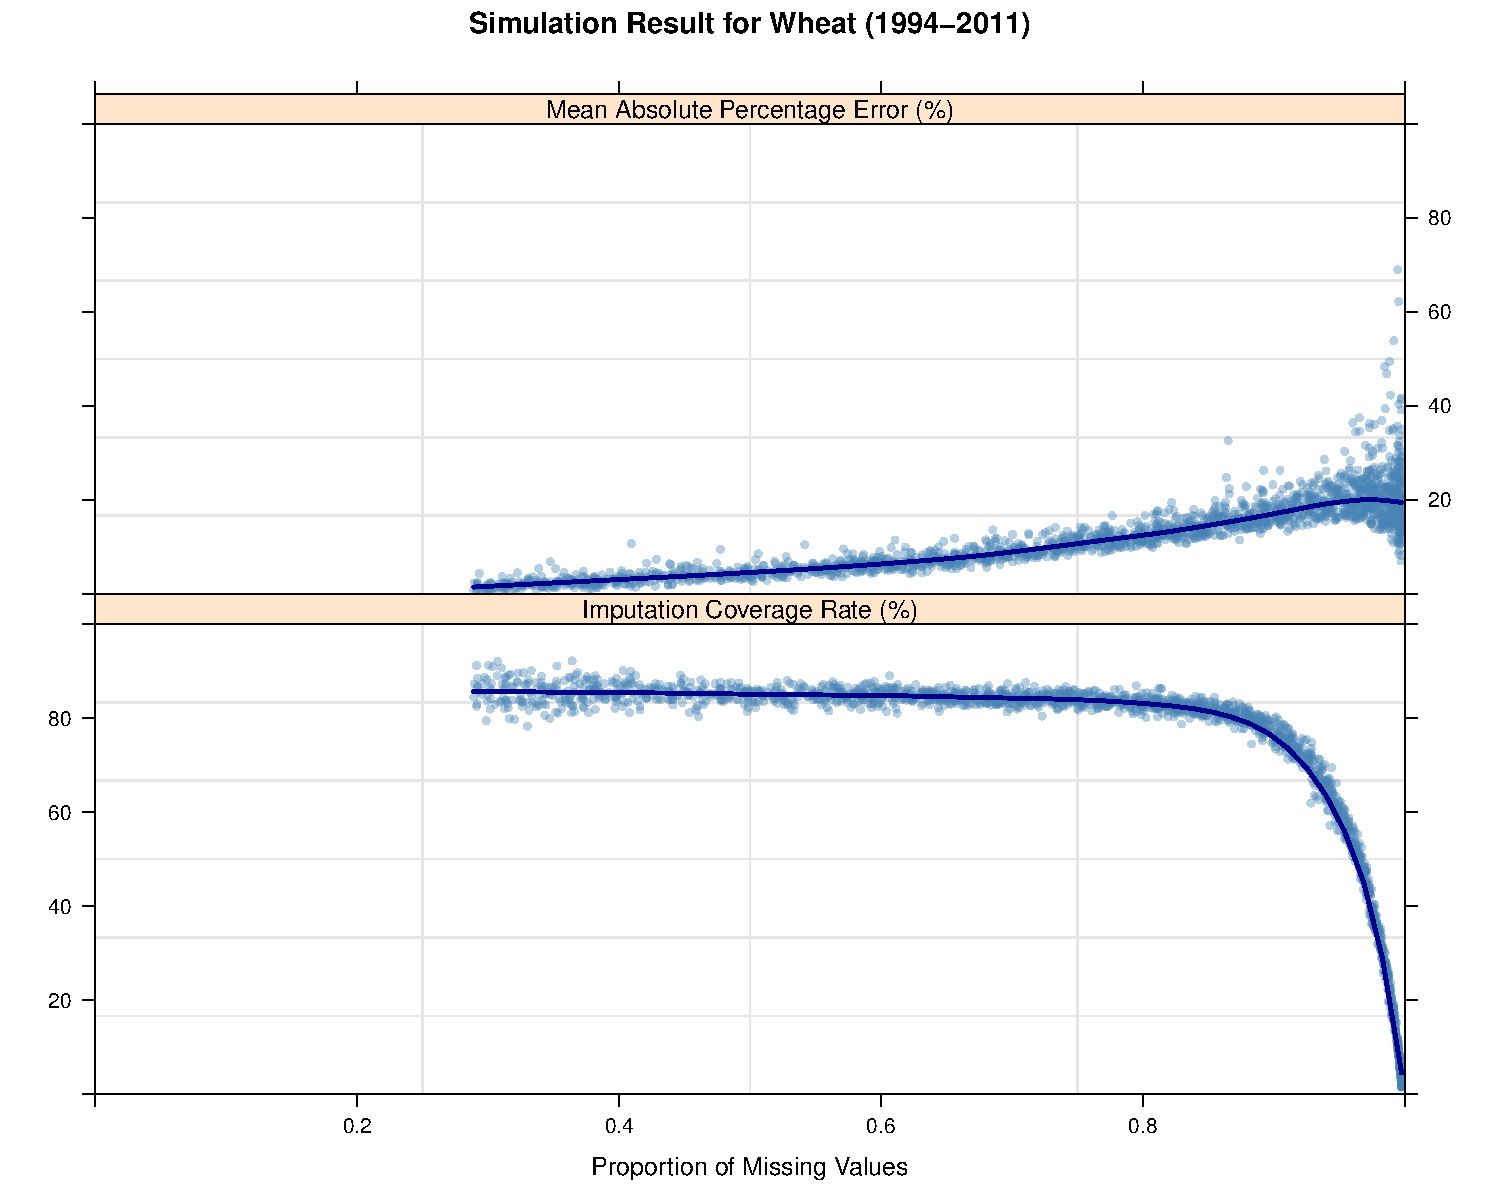
\includegraphics[width = \maxwidth]{wheatSimulationResult}
  \caption{Bootstrapped imutation error rate for wheat}
\end{figure}

\section{Conclusion and Future improvements}
The aim of the paper has been to overhaul the current imputation
methodology, with a more consistent, yet better performing approach.

The proposed model demonstrates the ability to resolve issues such as
diverging area and production series and biased growth as a result of
missing values. Furthermore, the proposal takes into account the
attribute of incorporating relevant information as well as
establishing a flexible framework to accommodate additional
information.

This is, however, work in progress, as the technical teams are
continuing to collaborate in order to seek a deeper understanding of
the data in order to improve on the model. Application of the
state-space model might be a candidate to succeed in this regard, as
it allows for production, area and yield to be imputed simultaneously.
In addition, additive mixed model are under-investigation for country
non-linearity departures.

\section{Acknowledgement}
This work is supervised by Adam Prakash with assistance from Nicolas
Sakoff, Onno Hoffmeister and Hansdeep Khaira whom were crucial in the
development of the methodology. The author would also like to thank
the team members which participated in the first round of the
discussion providing valuable feedbacks. Finally, credits to Cecile
Fanton and Frank Cachia whom devoted their time to translate the paper
into French.



\section*{Annex 1: Geographic and classification}

The geographic classification follows the UNSD M49 classification at
\url{http://unstats.un.org/unsd/methods/m49/m49regin.htm}. The
definition is also available in the \code{FAOregionProfile} of the R
package \pkg{FAOSTAT}.

\section*{Annex 2: Pseudo Codes}

\begin{algorithm}
  \SetAlgoLined
  \BlankLine
  Initialization\;
  \Indp\Indp\Indp 
  $\hat{Y}_{i, t} \leftarrow f(Y_{i, t})$\;
  $\cal{L}_{\text{old}} = -\infty$\;
  $\cal{E}$ = 1e-6\;
  n.iter = 1000\;
  \Indm\Indm\Indm

  (1) Estimate model without grouped average effect\;
  \Indp\Indp\Indp  
  $\hat{Y}_{i, t} \leftarrow \hat{\beta}_{0,j} + \hat{\beta}_{1,j}t +
  \hat{b}_{0i} + \hat{b}_{1i}t $\;
  \Indm\Indm\Indm
  
  (2) Estimate model with grouped average effect\;
  \Begin{
      \For{i=1 \emph{\KwTo} n.iter}{
        E-step: Compute the expected group average yield\;
        \Indp\Indp\Indp 
        $\bar{Y}_{j, t} \leftarrow 1/N \sum_{i \in j} \hat{Y}_{i}$\;
        \Indm\Indm\Indm 
        
        M-step: Estimate the Linear Mix Model in \ref{eq:lmeImpute}\;
        \If{$\cal{L}_{\text{new}} - \cal{L}_{\text{old}} \ge
          \cal{E}$}{ $\hat{Y}_{i, t} \leftarrow \text{fitted value of
            the model}$\; $\cal{L}_{\text{old}} \leftarrow
          \cal{L}_{\text{new}}$\; } \Else{ break } } }
    
    %% (3) Select model with the smallest AIC
    
    \caption{EM-Algorithm for Imputation}
    \label{alg:imputation}
\end{algorithm}
  
      

\begin{algorithm}[H]
  \SetAlgoLined
  \KwData{Production (element code = 51) and Harvested area (element
    code = 31) data}

  \KwResult{Imputation}
  
  \BlankLine
  Missing values are denoted $\emptyset$\;

  \BlankLine
  Initialization\;
  \Begin{
      \If{$A_t = 0 \land P_t \ne 0$}{
        $A_t \leftarrow \emptyset$\;
      }
      \If{$P_t = 0 \land A_t \ne 0$}{
        $P_t \leftarrow \emptyset$\;
      }
  }  
    
  \BlankLine  
  Start imputation\;
  \Begin{
      \ForAll{commodities}{
        
        (1) Compute the implied yield\;
        \Indp\Indp\Indp 
        $Y_{i,t} \leftarrow P_{i,t}/A_{i,t}$\;
        \Indm\Indm\Indm
                
        (2) Impute the missing yield with the imputation algorithm
        \ref{alg:imputation}\; \Indp\Indp\Indp
        
        %% $\hat{Y}_{i,t} \leftarrow \hat{\beta}_{0j} + \hat{\beta}_{1j}t
        %% + \hat{\beta}_{2j}\bar{Y}_{j,t} + \hat{b}_{0i} +
        %% \hat{b}_{1i}t$\;
        
        \Indm\Indm\Indm        
        
        \ForAll{imputed yield $\hat{Y}_{i, t}$}{
          \If{$A_t = \emptyset \land P_t \ne \emptyset$}{
            $\hat{A}_{i, t} \leftarrow P_{i, t}/\hat{Y}_{i, t}$\;
          }
          \If{$P_t = \emptyset \land A_t \ne \emptyset$}{
            $\hat{P}_{i, t} \leftarrow A_{i, t} \times \hat{Y}_{i, t}$\;
          }
        }
        
        (4) Impute area ($A_{i, t}$) with equation
        \ref{eq:linearInterpolation} then \ref{eq:locf}\;
        
        \ForAll{imputed area $\hat{A}_{i, t}$}{ \If{$\hat{Y}_{i, t}
            \ne \emptyset$}{ $\hat{P}_{i, t} \leftarrow \hat{A}_{i, t}
            \times \hat{Y}_{i, t}$\; } } } }
  \caption{Imputation Procedure}
\end{algorithm}

  
\section*{Annex 3: Supplementary Resources}

The data, code implementation and documentation can all be found and
downloaded from \url{https://github.com/mkao006/sws_imputation}. This
paper is generated on \today and is subject to changes and updates.
  
\begin{thebibliography}{9}
\bibitem{dougbates2010}
  Douglas M. Bates
  \emph{lme4: Mixed-effects modelling with R}
  2010
  
\bibitem{impWorkingPaper2011}
  Data Collection, Workflows and Methodology (DCWM) team,
  \emph{Imputation and Validation Methodologies for the FAOSTAT Production Domain}.
  Economics and Social Statistics Division,
  2011.
  
\bibitem{lairdWare1982}
  Nan M. Laird, James H. Ware,
  \emph{Random-Effects Models for Longitudinal Data}.
  Biometrics Volume 38, 963-974,
  1982.
  
\bibitem{rCore}
  R Core Team,
  \emph{A language and environment for statistical computing.}
  R Foundation for Statistical Computing, Vienna, Austria.
  ISBN 3-900051-07-0, URL http://www.R-project.org/,
  2013.
  
\bibitem{nlme}
  Jose Pinheiro, Douglas Bates, Saikat DebRoy, Deepayan Sarkar and the
  R Development Core Team,
  \emph{nlme: Linear and Nonlinear Mixed Effects Models.} 
  R package version 3.1-108.
  2013

\bibitem{lme4}
  Douglas Bates, Martin Maechler, Ben Bolker and Steven Walker (2013).
  \emph{lme4: Linear mixed-effects models using Eigen and S4.} 
  R package version 1.0-4. http://CRAN.R-project.org/package=lme4
 
\bibitem{rubin1976}
  Donald B. Rubin,
  \emph{Inference and Missing Data},
  Biometrika, Volume 63, Issue 3, 581-592,
  1976
  
\bibitem{unido2012}
  Valentin Todorov, Matthias Templ
  \emph{R in the Statistical Office: Part II}
  2012
  
\bibitem{laird_ware1982}
  Nam M. Laird, James H. Ware
  \emph{Random-Effects Models for Longitudinal Data}
  Biometrics, Volume 38, Number 4, pp.963-974
  1982

\bibitem{dempster_laird_rubin1977}
  A. P. Dempster, Nam M. Laird, D. B. Rubin
  \emph{Maximum Likelihood from Incomplete Data via the EM Algorithm}
  Journal of Royal Statistical Society. Series B (Methodological), Volume 39, Number 1, pp1-38
  1977
  
\bibitem{lai_huang_lee2012}
  Randy C. S. Lai, Hsin-Cheng Huang, Thomase C. M. Lee
  \emph{Fixed and random effects selection in nonparametric additive mixed models}
  Electronic Journal of Statistics, Volume 6, pp810-842
  2012
\end{thebibliography}
  



\end{document}
